\documentclass[12pt]{article}
\usepackage[numbers]{natbib}
\usepackage[margin=1in]{geometry}
\usepackage[nottoc]{tocbibind}
\usepackage{graphicx}

\graphicspath{{../images}}

\author{Thomas Kwashnak}
\title{DS-480 Project}

\begin{document}

\maketitle

\newpage

\section{Abstract}

\section{Introduction}


% Board Ideas

\paragraph{}
Reinforcement learning is a subset of machine learning that aims to complete a goal in an environment.
This can range from solving a maze, to playing a video game, to learning how to drive a car.
Regardless of the environment, the goal of the reinforcement learning agent is to find a policy, or a mapping of all possible states to the actions the agent takes, that will maximize some long-term reward \cite{article_reinforcement_learning_survey}.
An agent does this by learning the Q-Values associated with the environment, or the estimated reward for taking some action $A$ at a state $S$.
This method alone is infeasable for more complicated environments, where accounting for every move in every possible state is nearly impossible to represent, or would take too long to train.
Deep-Q Learning provides a solution by using a neural network to \textit{estimate} the Q-Values of each action given the current state \cite{article_human_level_control_deep_reinforcement_learning}.

% Remaining Issues
\paragraph{}
Simple back propagation techniques, used to train and modify neural networks, can often run into the issue of requiring a lot of time to train \cite{article_accelerating_neural_networks_weight_extrapolations}.
As the data sets we use get bigger and more complex, the longer it takes for models to train and accurately model the patterns presented.
Deep-Q learning models are no different.
Additionally, some environments may have many states with no reward and few states with positive or negative reward.
This means that agents must take more steps before finding a positive or negative reward, and can lead agents to mindlessly exploring before finding any reward \cite{article_approx_optimal_approximate_reinforcement_learning}.

% Project Details

\paragraph{}
This paper explores a potential training improvement for deep reinforcement learning models in environments with large state space and a known goal.
The idea is that an agent learning to back-track its own steps is faster than exploring the whole environment.
First, the agent will be given a smaller state-space closer to the end-goal, and then expanded over time to allow the agent to learn the entire maze.
The agent will be trained alongsize control agent to compare the ability each agent has to solve the maze over their training time.
The data collected will be able to suggest whether this training strategy improves the training rate of the model.

\section{Methods}


\subsection{Environment}
\paragraph{}

In this project, the task of the agent is to explore a simple maze.
The maze is stored as a 2-dimensional array of locations, which can either be empty or filled in.
The maze itself is generated and stored using mazelib \cite{lib_mazelib} in Python \cite{lang_python}.
The output of the environment consists of the maze configuration, the current location, and the target goal.
The maze configuration is represented by a flattened array representing empty ($0$) spaces and walls ($1$).
The current position and goal position are stored as their x and y coordinates using $n * m$ variables.
Similar to the configuration, 

% The environment that the agent explores is a simple maze.
% The maze itself is generated and stored using the python library mazelib \cite{lib_mazelib}.
%
% The environment that the agent explore is a simple maze.
% The maze consists of a 2-dimensional array of empty spaces and walls.
% The environment output given to the agent contains both the maze and the agent's position.
% The maze is encoded in $0$s and $1$s, representing empty spaces and walls respectively.
% This is given for every tile on the map.
% The agent's position will be given by its X and Y coordinates, encoded into a binary format.

\subsection{Reinforcement Learning Model}

\subsection{Agent Training}

\subsection{Data Collection}


% \subsection{Environment}
% \paragraph{}
% % Alternatively this may be encoded as 00100 00010 etc.
% The agent is placed at a random point in the maze, and its goal is to reach the top left corner $(0,0)$
%
% % % \subsection{Reinforcement Learning Model}
%
% % % \paragraph{}
% % % The agent will be implemented and trained based on a simple Deep-Q machine learning model \cite{article_reinforcement_learning_survey}.
%
% % \subsection{Agent Specifications}
%
%
% \subsection{Data Collection and Analysis}
% \paragraph{} Data is collected from the script into a CSV file. The data is then analyzed using Tidyverse \cite{lib_tidyverse}, and graphs are created using ggplot2 \cite{lib_ggplot2}


\section{Results}

\paragraph{} 
The two models were trained on identical datasets.
In total, $10,000$ observations were recorded for each model. 
Each model was given the same observations and dataset, and trained in the same manner.

\begin{figure}[h]
    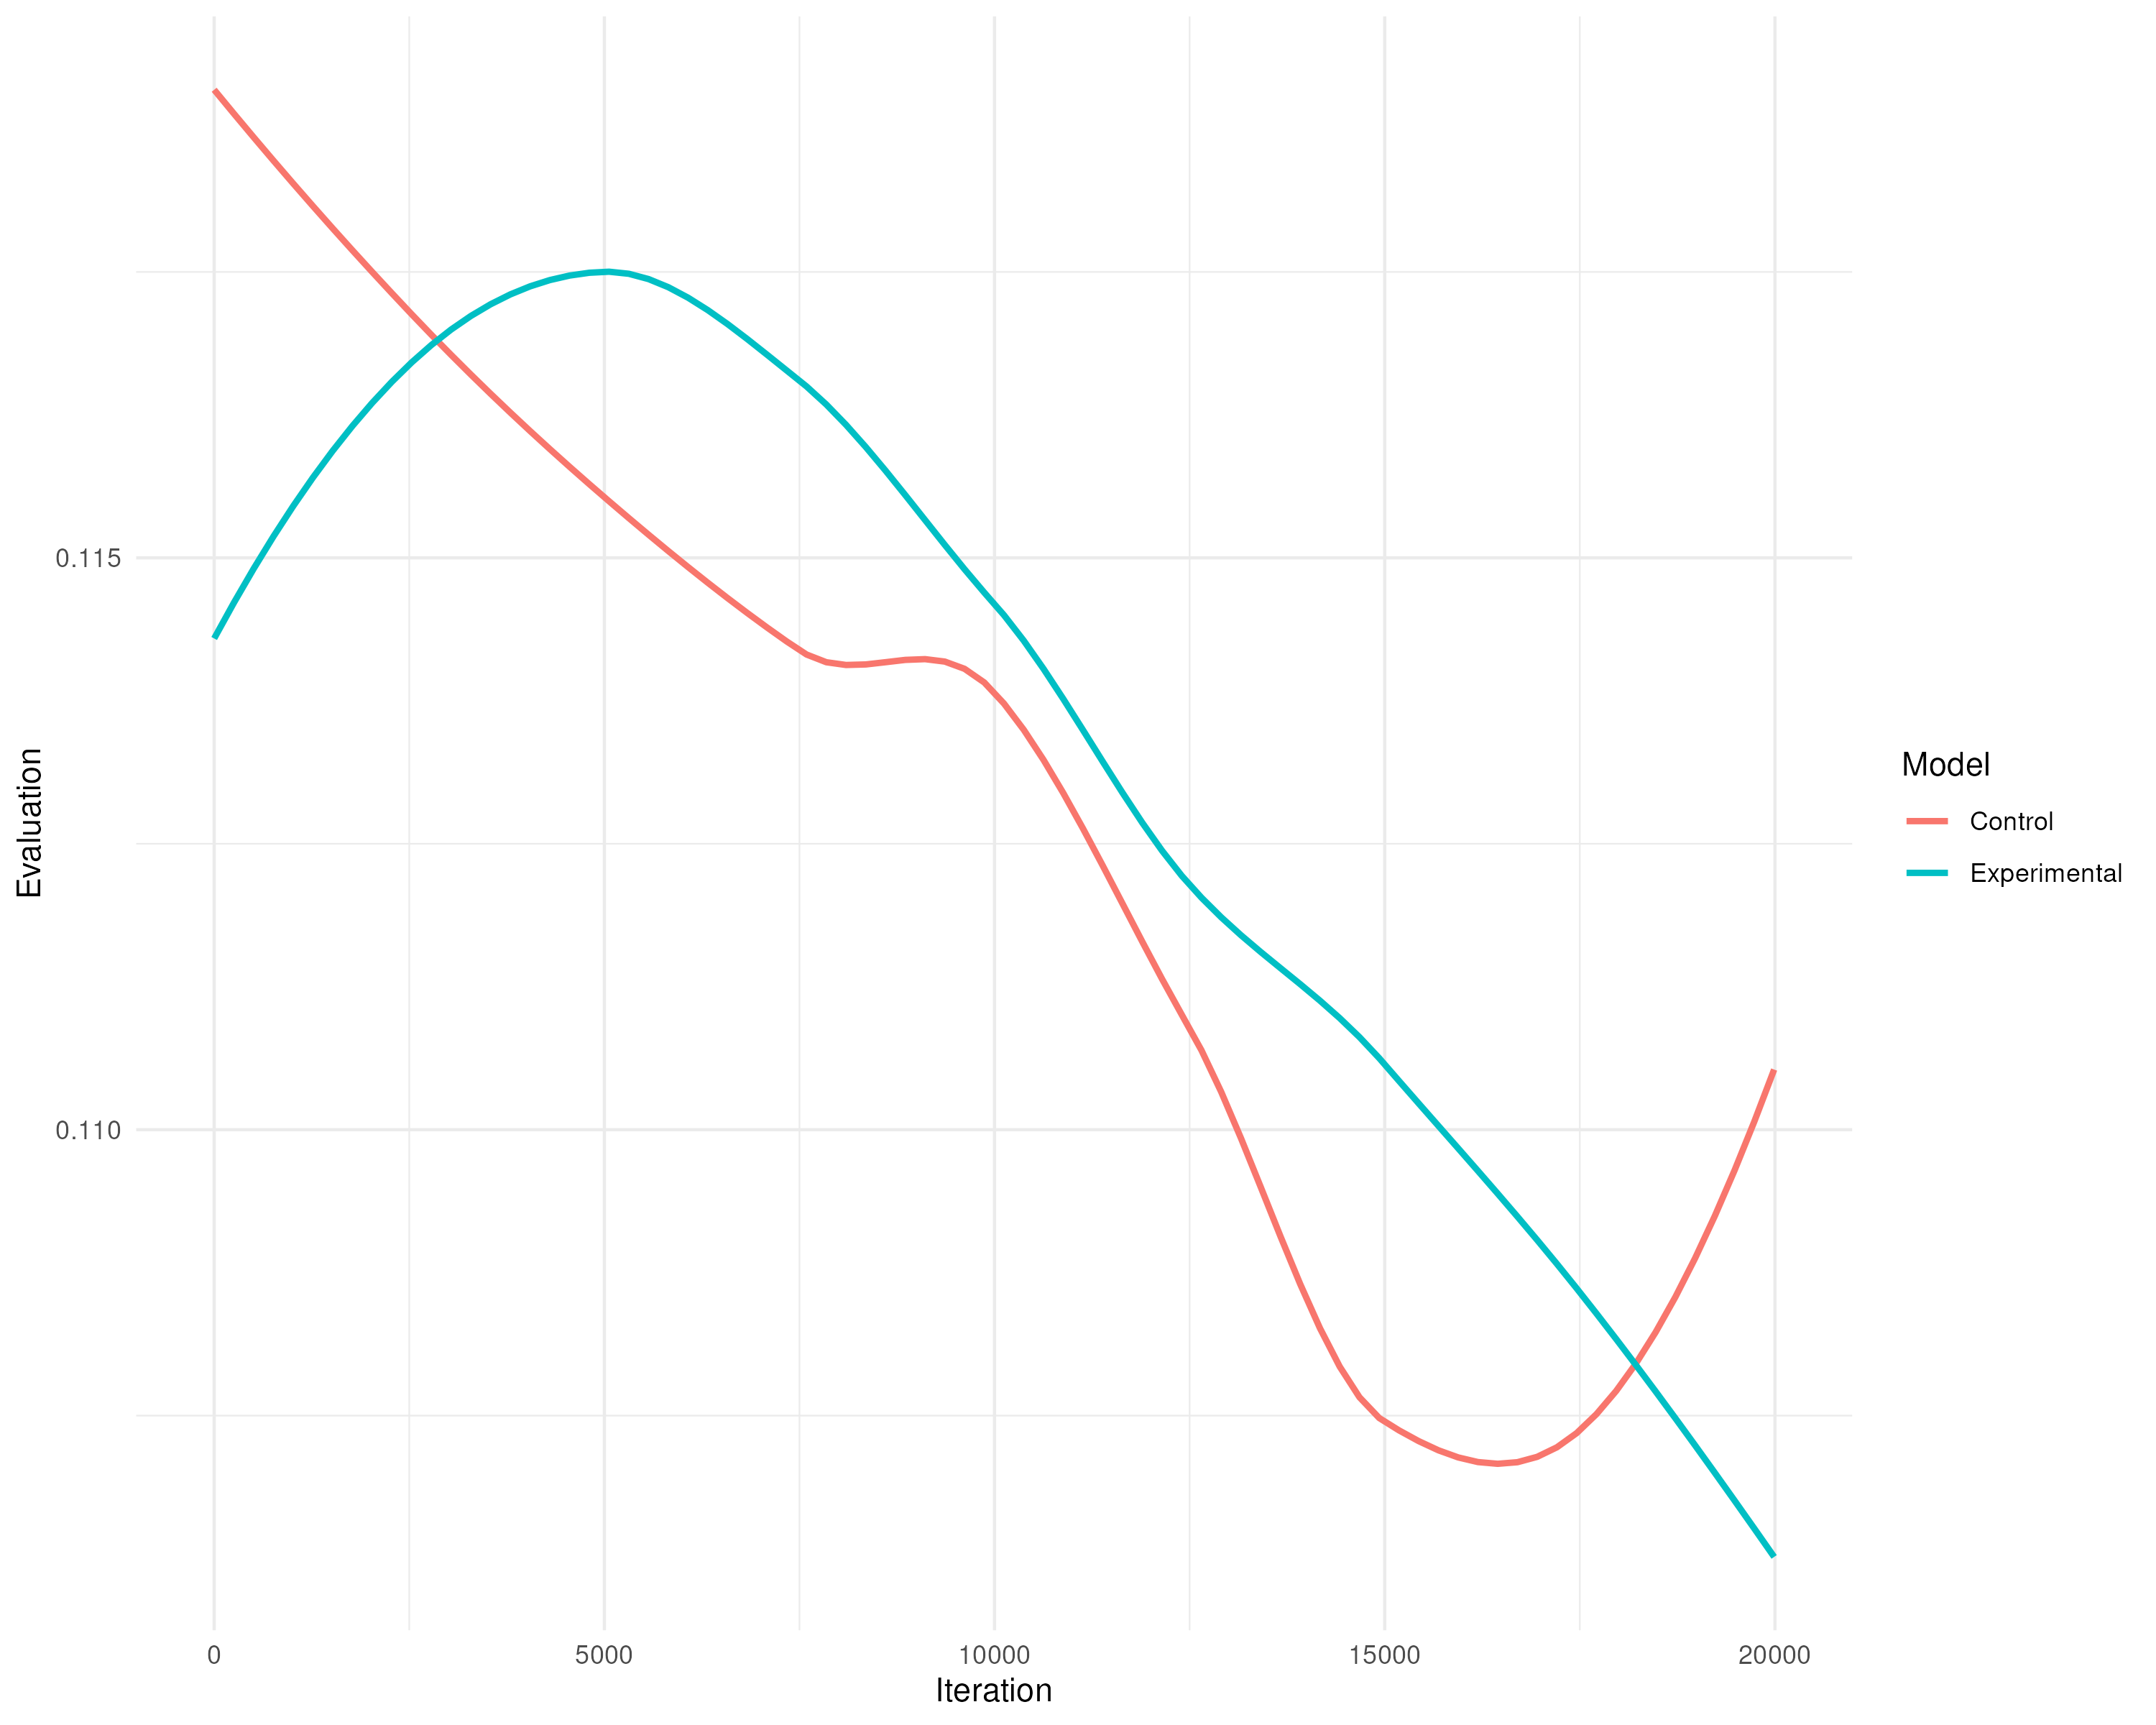
\includegraphics[width=\linewidth]{graph.png}
    \caption{Model evaluation over time. Evaluation is calculated from the policy generated by the agent, represented as the percent of the maze that the policy successfully reaches the end from (higher is better).}
		\label{fig:graphs}
\end{figure}

\paragraph{}
Figure \ref{fig:graphs} shows the model evaluation throughout the training.
The control model did not change it's policy at all, so it maintained a consistent Evaluation level.
The experimental model has two distinct properties.
First, it has signicicantly lower evaluations than the control model.
At no point during the training did the experimental model obtain a higher evaluation than the control model.
Second, the model shows an initial dip in it's evaluation during the first $500$ iterations.
Afterwards, it slowly climbs back up, but never higher than it had in the first few iterations.




\newpage
\bibliographystyle{ieeetr}
\bibliography{refs}

\end{document}
